
\begin{minipage}[c]{\textwidth}
\centering
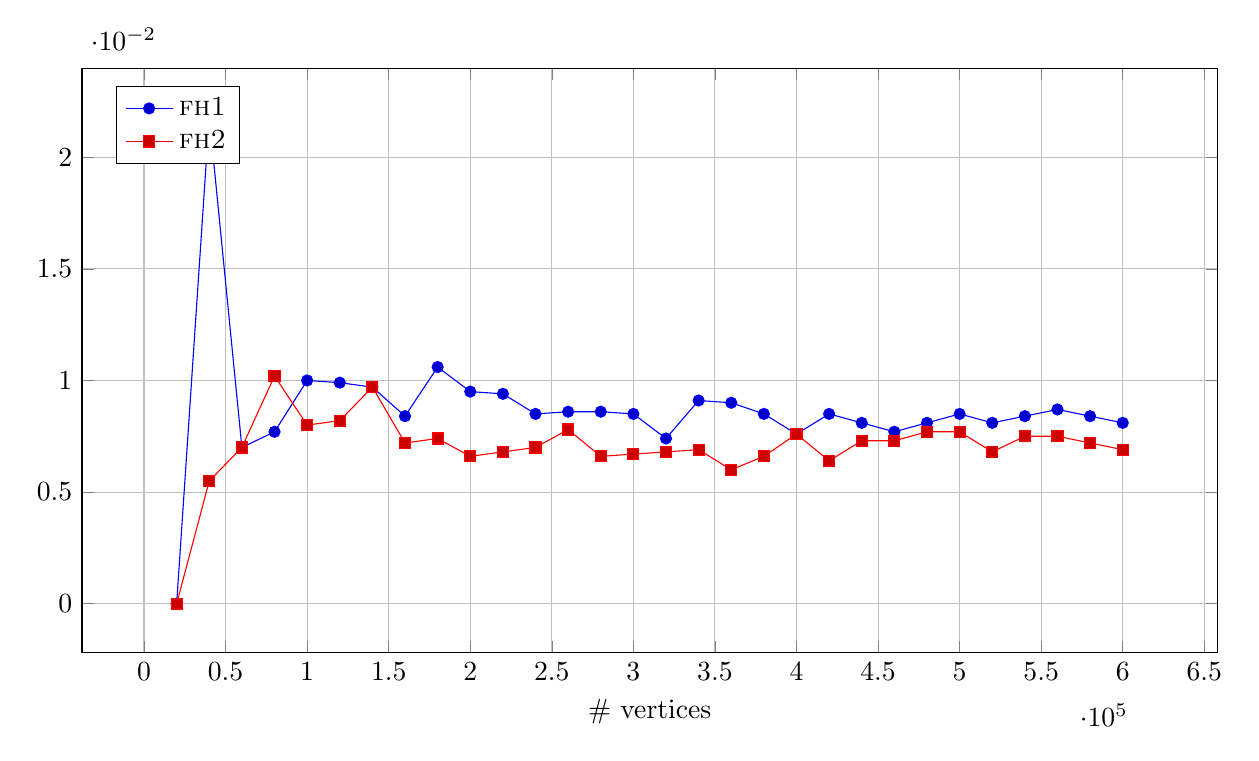
\begin{tikzpicture}
        \begin{axis}[
            xlabel = \# vertices,
            height=9cm,
            width=16cm,
            grid=major,
            legend pos=north west
    	]

        \addplot coordinates {
(20000,0.0000)
(40000,0.0218)
(60000,0.0070)
(80000,0.0077)
(100000,0.0100)
(120000,0.0099)
(140000,0.0097)
(160000,0.0084)
(180000,0.0106)
(200000,0.0095)
(220000,0.0094)
(240000,0.0085)
(260000,0.0086)
(280000,0.0086)
(300000,0.0085)
(320000,0.0074)
(340000,0.0091)
(360000,0.0090)
(380000,0.0085)
(400000,0.0076)
(420000,0.0085)
(440000,0.0081)
(460000,0.0077)
(480000,0.0081)
(500000,0.0085)
(520000,0.0081)
(540000,0.0084)
(560000,0.0087)
(580000,0.0084)
(600000,0.0081)

    	};
        
    	\addlegendentry{\textsc{fh1}}

        \addplot coordinates {
(20000,0.0000)
(40000,0.0055)
(60000,0.0070)
(80000,0.0102)
(100000,0.0080)
(120000,0.0082)
(140000,0.0097)
(160000,0.0072)
(180000,0.0074)
(200000,0.0066)
(220000,0.0068)
(240000,0.0070)
(260000,0.0078)
(280000,0.0066)
(300000,0.0067)
(320000,0.0068)
(340000,0.0069)
(360000,0.0060)
(380000,0.0066)
(400000,0.0076)
(420000,0.0064)
(440000,0.0073)
(460000,0.0073)
(480000,0.0077)
(500000,0.0077)
(520000,0.0068)
(540000,0.0075)
(560000,0.0075)
(580000,0.0072)
(600000,0.0069)

    	};
        
    	\addlegendentry{\textsc{fh2}}


        \end{axis}

    \end{tikzpicture}
    \captionof{figure}{Running time divided by $nlogn$}
    \label{fig:time_16}
\end{minipage}
